There are two panels in this application.
On the left is the ``Input" panel, where the user can load an experiment, configure the finite element model, and run analysis.
On the right is the ``Output" panel, where the user see results visualized, such as the mesh of the wall, the hysteric curves, etc.


The first step to load an existing experiment. By default, a demo experiment will be loaded automatically. 
The description of an experiment consists three json files: BIM.json, EVT.json and EDP.json \Cref{fig:demos}. 
BIM.json describes the geometry and the material of the shear wall.
EVT.json describe the loading applied to the wall. EDP.json describes the response of the wall to the loading. 
The user can find these demo files inside the directory that contains the executable of the application. 
When the user have their own experimental data prepared in this manner, they can click the button ``Add Experiment" to loaded.


\begin{figure}[!htbp]
  \centering {
    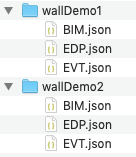
\includegraphics[width=0.2\textwidth]
    {figures/SWIM_demos.png} }
  \caption{Experiment files}
  \label{fig:demos}
\end{figure}

When an experiment data is loaded successfully, the ``Wall info" tab will show up \Cref{fig:bim}.
Where the user can choose to display the information of each floor, view the geometry, the material being used, and the layout of the reinforcement bars.
No edit is allowed in this tab, because this shall be the description of the experiment which is a fact.

\begin{figure}[!htbp]
  \centering {
    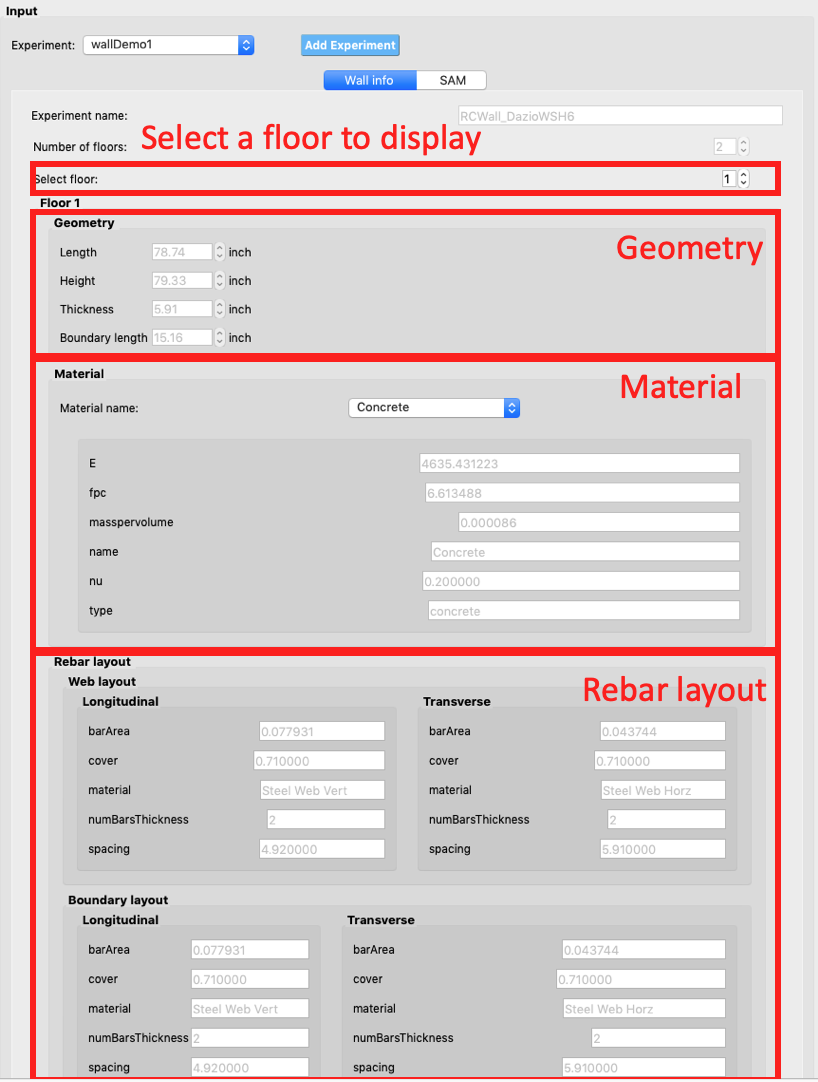
\includegraphics[width=0.8\textwidth]
    {figures/SWIM_input.png} }
  \caption{The ``Wall info" tab}
  \label{fig:bim}
\end{figure}

While the experiment being loaded, the application will automatically process the data and pick up suitable material models to show in the ``SAM" tab.
Meanwhile, the geometry of the wall will be displayed on the right of the application.
Inside the ``SAM" tab, the users can edit to control the mesh density and the parameters of the material model \Cref{fig:sam}. 


\begin{figure}[!htbp]
  \centering {
    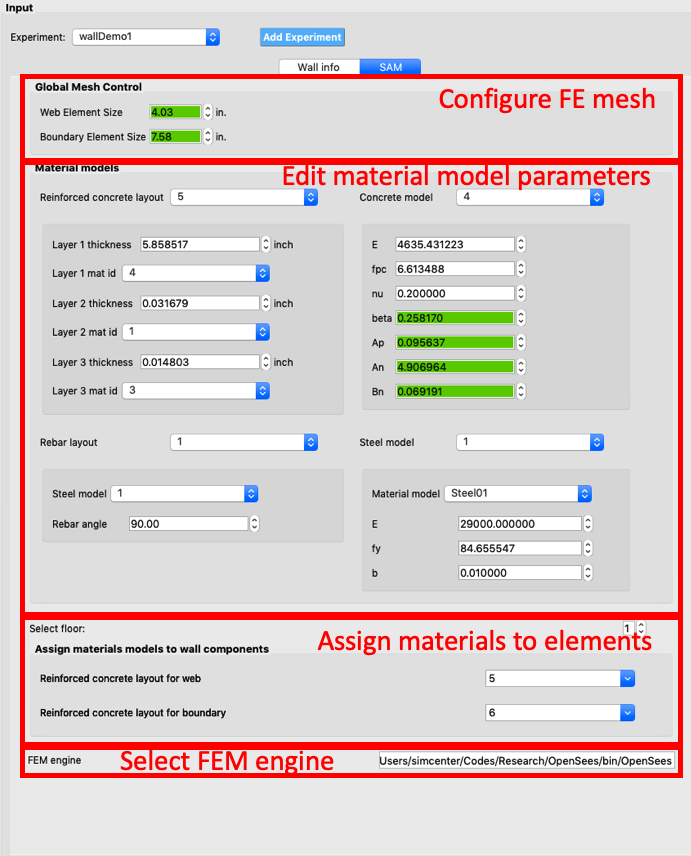
\includegraphics[width=0.8\textwidth]
    {figures/SWIM_SAM.png} }
  \caption{The ``SAM" tab}
  \label{fig:sam}
\end{figure}




In the ``Global Mesh Control" section inside the SAM tab, users can specify the element size of the finite element mesh. 
By default, the mesh sizes are set to be maximum values, so that the user can see the geometry of the wall rendered in grey color in the ``Shape" section on the right  \Cref{fig:shape} (a). 
When the use edit the sizes, the geometry will be replaced with element mesh rendered in blue \Cref{fig:shape} (b). 
If the user click the AI button at the bottom of the Input panel, the geometry will be replaced by green colored elements generated by AI \Cref{fig:shape} (c).

\begin{figure}[!htbp]
  \centering 
  \subfloat[Wall geometry]{
    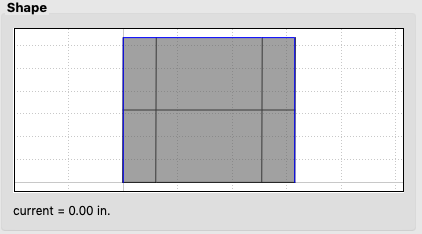
\includegraphics[width=0.39\textwidth]
    {figures/SWIM_shape_1.png}}
  \subfloat[User specified mesh]{
    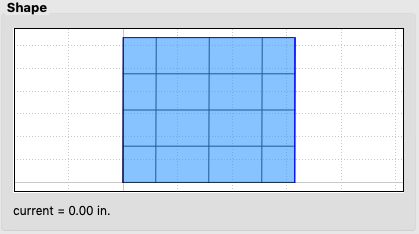
\includegraphics[width=0.39\textwidth]
    {figures/SWIM_shape_2.png}}
    
    \subfloat[Mesh generated by AI]{
    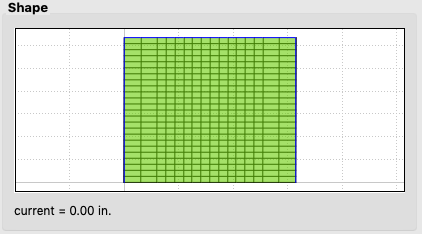
\includegraphics[width=0.39\textwidth]
    {figures/SWIM_shape_3.png}}
  \caption{Shape and mesh visualization}
  \label{fig:shape}
\end{figure}


While the AI button being clicked, several parameters will be edited by AI, including:
\begin{enumerate}
\item Web Element Size
\item Boundary Element Size
\item beta (Concrete model)
\item Ap (Concrete model)
\item An (Concrete model)
\item Bn (concrete model)
\end{enumerate}
Their color will be changed to green indicating these are AI predicted values \Cref{fig:colors}.
When the user try to edit these values, their color will be returned to white, 
while the mesh color being returned to blue \Cref{fig:shape} (b), 
indicating these settings are set by the user.

\begin{figure}[!htbp]
  \centering 
  \subfloat[Default settings]{
    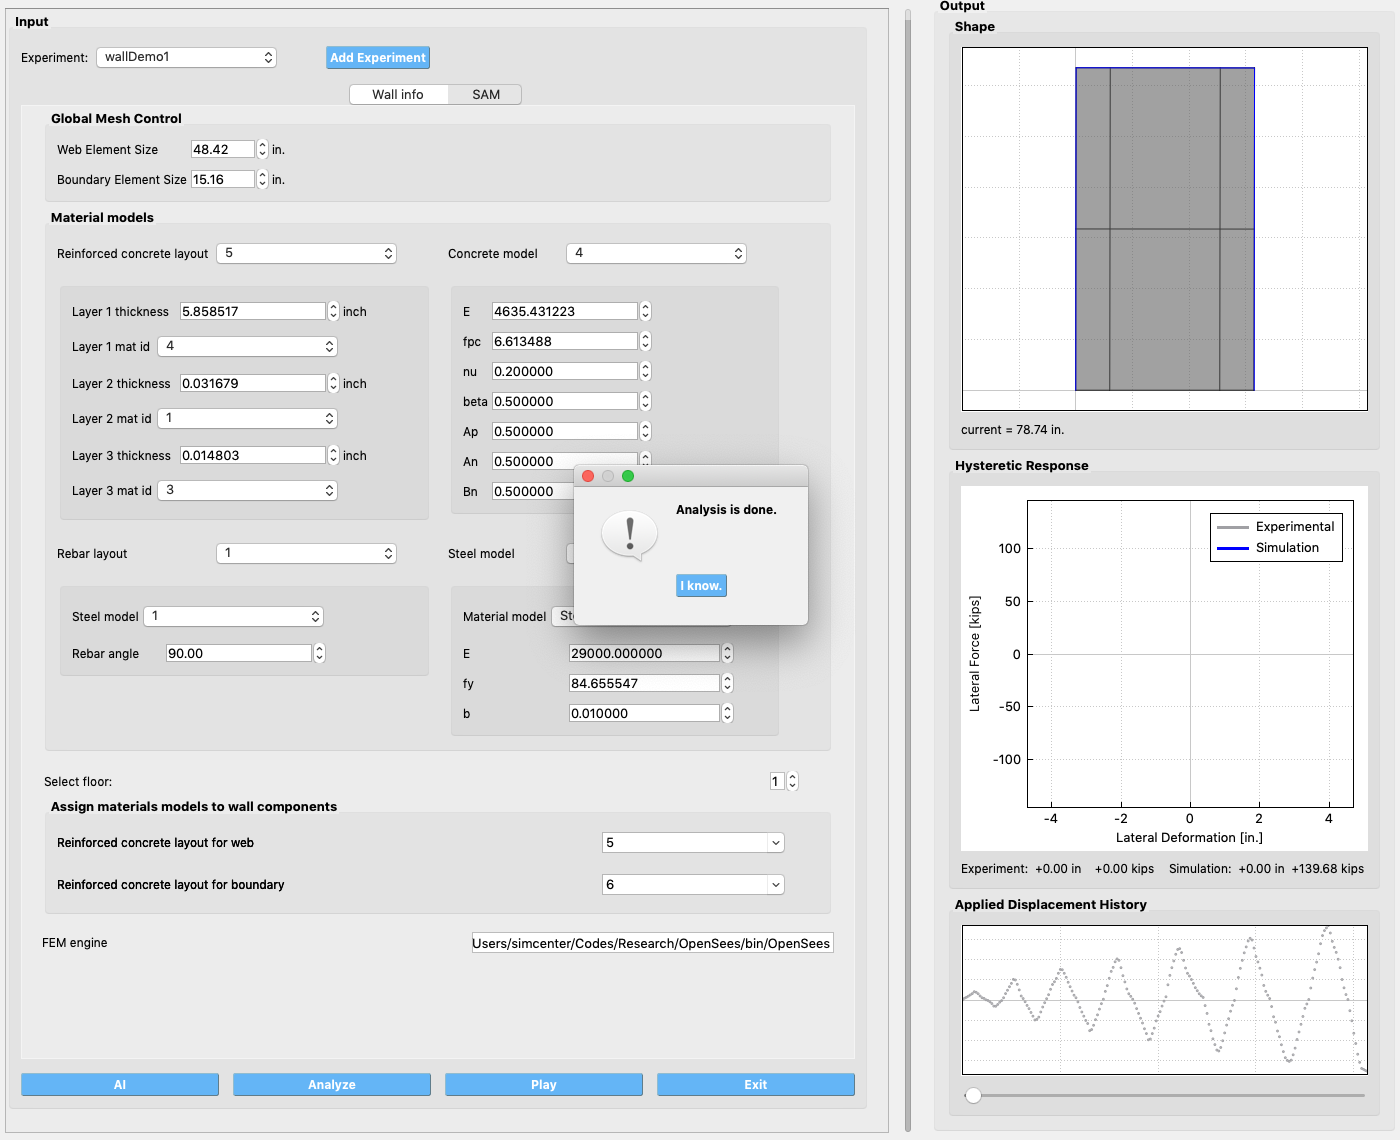
\includegraphics[width=0.47\textwidth]
    {figures/SWIM_grey.png}}
  \subfloat[AI settings, colored in green]{
    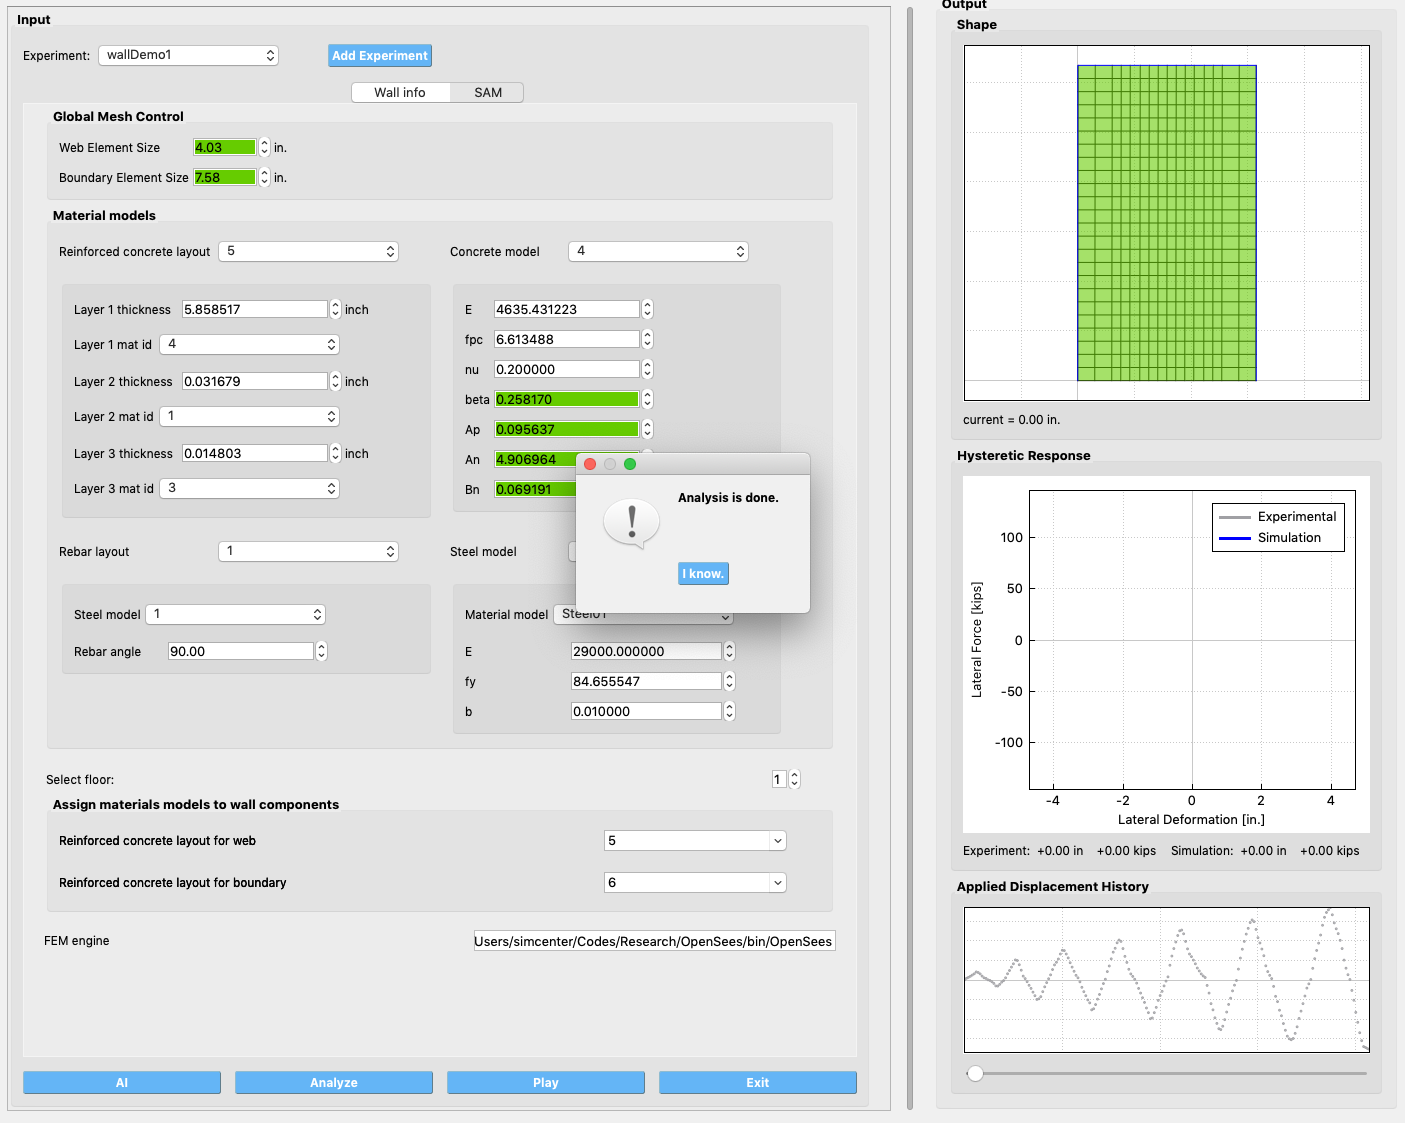
\includegraphics[width=0.48\textwidth]
    {figures/SWIM_green.png}}

  \caption{Call AI}
  \label{fig:colors}
\end{figure}

At the bottom of the SAM tab, the user need to provide the path of a finite element program. 
This version only support OpenSees. 

Once the users finished the editing, they can click ``Analyze" button. 
This will bring up a progress bar shown between the Input and Output panels.
When the analysis is completed, a message windows will pop up. The user can click ``I know.", then click ``Play'' button.
The animations will start in the Output panel, including:
the deformed mesh, the hysteretic curves and the load history. 

\begin{figure}[!htbp]
  \centering {
    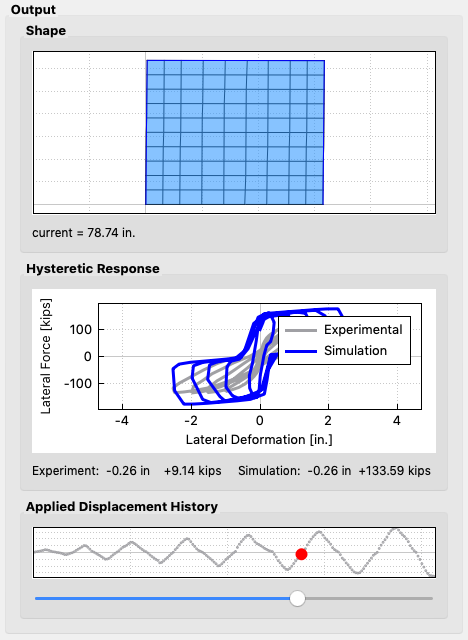
\includegraphics[width=0.8\textwidth]
    {figures/SWIM_output.png} }
  \caption{ Output tab}
  \label{fig:output}
\end{figure}

%Select a soil layer by clicking on the design table or by clicking on the graphic soil column.
%When a layer is selected, it will be highlighted in both the design table and the graphic. 
%In the design table, it is highlighted by changing the background color to light green. 


%Given that the properties of the soil layers and the earthquake events are known,
 %\texttt{\getsoftwarename{}} convert provide multiple nonlinear material models for simulating the soil behavior under earthquake loading.
